\documentclass[a4paper, 12pt, notitlepage]{article} % Style du document
%\usepackage[fontsize=13pt]{scrextend} %  Pour utiliser d'autres tailles de polices (Latex est susceptible sur ce point)
\usepackage[margin=1.3in]{geometry} % Petite marge
\usepackage[francais]{babel} % Langue du document

\usepackage[utf8]{inputenc} % Codage du fichier
\usepackage[T1]{fontenc} % Pour bien gérer les accents

\usepackage{cmbright} % Police utilisée

\usepackage{graphicx} % Pour pouvoir placer des images

\usepackage{xspace} % Gère les espaces après les commandes
\usepackage{hyperref} % Pour ajouter des liens dans le document
\usepackage[french]{varioref}
\hypersetup{
  colorlinks, 
  linktoc=all, 
  citecolor=black, 
  linkcolor=black, 
  urlcolor=black, 
  pageanchor=false
}

% Pour pouvoir utiliser des couleurs
\usepackage{xcolor}
% Définition des couleurs du thème Paris-Sud (couleurs du logo)
\definecolor{bleuPS}{HTML}{004870}
\definecolor{vertPS}{HTML}{84b818}
\definecolor{grisPS}{HTML}{6b6c6e}

\setlength{\parskip}{0.6 ex} % Ajoute un peu d'espace entre les paragraphes
\usepackage{titlesec} % Contre le changement d'espace dans les sections
\titlespacing*{\section}{0pt}{2.5 ex}{1 ex}
\titlespacing*{\subsection}{0pt}{2.5 ex}{1 ex}

\usepackage[ampersand]{easylist} % Pour faire des liste facilement
\newcommand\itemizeTrait{\ListProperties(Space=0 ex, Space*=0 ex, Style*=-- )} % Liste simple
\newcommand\itemizePuce{\ListProperties(Space=0 ex, Space*=0 ex, Style*=$\bullet$\ , Style2*=$\bullet$\ )} % Liste à puce

\usepackage{microtype} % Pour un texte bien mieux justifié

% Pour ajouter des pieds de pages
\usepackage{fancyhdr}
\pagestyle{fancy}
% Création des pieds de pages
\fancyhf{}
\lfoot{\textcolor{grisPS}{BestProjetGLA}}
\cfoot{\thepage}
\rfoot{\textcolor{grisPS}{Année 2016-2017 L3 Informatique}}
\renewcommand{\headrulewidth}{0pt}
\renewcommand{\footrulewidth}{1pt}
%\renewcommand{\footrule}{\hbox to\headwidth{\color{grisPS}\leaders\hrule height \footrulewidth\hfill}}
    
% Changement de couleurs des sections, sous-sections etc.
\usepackage{sectsty}
\sectionfont{\color{bleuPS}}
\subsectionfont{\color{vertPS}}
\subsubsectionfont{\color{grisPS}}

% Juste pour mettre du texte random en attendant d'écrire
\usepackage{lipsum}

% utile
\usepackage{subfig}
\graphicspath{{Images/}}
\usepackage{caption}
\DeclareCaptionType{maquetteFig}[Maquette][Table des maquettes]
\DeclareCaptionType{umlFig}[Diagramme UML][Table des diagrammes UML]


\usepackage{longtable}

\begin{document}

% Création de la page de garde
\begin{titlepage}
	\centering
	
\includegraphics[width=0.2\textwidth]{LogoUPSUD_ParisSaclay.jpg}\par\vspace{1cm}
	{\scshape\large Projet Génie Logiciel Avancé L3 \par}
	\vspace{1cm}
	{\scshape\large Cahier des charges\par}
	\vspace{1.5cm}
	{\huge\bfseries Assistant événementiel de sorties\par}
	\vspace{2cm}
	{\large CHOUKCHOU BRAHAM Abbes \\
					NDIAYE Thierno Ismaila\\
					VACHAUDEZ Cédric\par}

	\vfill

	Professeurs :\par NGUYEN VAN Hai\\FAISSOLE Florian

	\vfill

	{\large Année 2016-2017 L3 Informatique\par\par}
\end{titlepage}

% Table des matières non numéroté et sans pied de page
\pagenumbering{gobble}
{
\setlength{\parskip}{0 ex}
\tableofcontents
\thispagestyle{empty}
\newpage

%\vspace*{\fill}
\listofmaquetteFig
%\vspace*{\fill}
\vspace{1cm}
\listofumlFig
%\vspace*{\fill}
\thispagestyle{empty}
}
\newpage
\pagenumbering{arabic}


\newpage
\pagenumbering{arabic}

\section{Contexte}
Avant la démocratisation d'internet, rechercher le numéro de téléphone d'un ami ou l'adresse d'un restaurant pouvait vite devenir long et fastidieux dès lors que l'annuaire ne le contenait pas. Aujourd'hui, le premier réflexe pour trouver ce type d'information est de lancer une recherche sur internet. Aussi, avec l'avancée des technologies de l'information et de la communication portée par l'avènement des réseaux sociaux, nous gardons un contact permanent avec ceux qui nous sont proches et pouvons échanger avec des personnes d'horizons divers un peu partout dans le monde. Ainsi on assiste à l'explosion quantitative des données numériques, permettant d'obtenir de plus en plus d'informations de très bonne qualité sur chaque personne et chaque lieu qui nous entourent.
Pourquoi ne pas utiliser cette immense banque de données pour organiser la rencontre entre plusieurs groupes de personnes (la famille, les amis, les collègues...) dans différents types d'endroits et qu'ainsi tout le monde puisse s'y retrouver ?

\section{Motivation}
Malgré la quantité de données et de moyens de communications disponibles aujourd'hui, il n'existe hélas aucun logiciel permettant de totalement automatiser l'organisation d'une soirée entre amis. Serte beaucoup d'applications aident à s'organiser, mais elles se limitent souvent à quelques fonctions de recherche et d'organisation là où les moyens actuels pourraient permettre de tout automatiser.

\subsection{Problématique}
La vie et ses multiples changements nous amènent à nous séparer de notre famille ou de nos amis et nous font manquer de bons moments. Il est donc primordial qu'au moment de revoir notre famille ou nos amis, tout se déroule sans accroc.
Notre but sera donc de créer une application permettant, le plus simplement possible, d'organiser sa soirée en suivant les étapes suivantes :
\begin{easylist}[itemize] \itemizeTrait
& On crée un événement (retrouvailles, promenades, dîners, rencontres de travail...).
& On ajoute dans l'application les trois participants à la soirée, leurs adresses et leurs goûts alimentaires (Julie DETESTE les kebabs).
& On choisit ce que l'on souhaite faire (aller manger, puis papoter dans un bar avant de partir en boîte).
& On valide, et l'application nous propose sans autre interaction de notre part l'itinéraire le plus rapide permettant d'effectuer ces trois activités en prenant en compte les durées des trajets, les goûts des participants et les horaires d'ouvertures des différents lieux concernés.
\end{easylist}

\subsection{État de l'art}
Gérer et organiser une rencontre requiert une bonne planification et exige de prendre en considération plusieurs critères parmi lesquels le budget, le lieu de résidence, les moyens de transport, les préférences de tout un chacun.
Il existe actuellement de nombreuses applications et sites répondant à des besoins similaires aux nôtres sur certains points, mais on pourra aussi énumérer plusieurs différences avec la nôtre.

On peut par exemple utiliser des sites ou applications permettant de planifier les soirées et de faire voter les participants (\href{http://ziwego.com/fr}{Ziwego}, Wepopp (non maintenue actuellement), \href{http://doodle.com/fr/}{Doodle} ou tout agenda électronique tel que Google event), mais c'est alors à l'utilisateur de créer, organiser et enregistrer le déroulement de sa soirée. Étape principale et fastidieuse que notre application nous dispensera d'effectuer.

Il est aussi possible de trouver des sites et applications pour obtenir des informations sur des restaurants, cinémas, bars etc. Citons entre autre \href{https://www.tripadvisor.fr/}{TripAdvisor}, \href{http://www.allocine.fr/}{Allociné}, ou tout simplement Google Map.
Tous ces logiciels et sites utilisent pour renvoyer les informations recherchées différentes API, accessibles gratuitement ou non, quand ce ne sont pas leurs propres bases de données. Notre application se servira dans plusieurs de ces bases de données, remplaçant donc le travail de recherche que l'utilisateur aurait dû effectuer avant.

Aussi il existe des outils qui permettent d'organiser des rencontres entre amis de manière plus originale (comme StrokeSurvey), permettant d'organiser un événement suite à la rédaction d'une proposition de sortie, à la sélection des dates préférentielles et à l'envoi par mail de différentes invitations à ses amis. La réussite d'un tel événement repose donc sur la réponse des différents participants et cela peut prendre un certain temps et causer l'échec de l'événement. Notre application ne pouvant disposer de son propre serveur, il nous sera impossible d'intégrer ce type de possibilité.

Enfin, certaines sociétés proposent d'organiser des événements de A à Z, mais le coût est élevé car c'est un travail réalisé par des humains et non par un simple logiciel. Ce sont donc des solutions réservées aux entreprises, à l'image de \href{http://www.baladenigm.com/}{BaladEnigm Business Events} qui permet d'organiser différents types d'événements entre collègues avec notamment la tenue de jeux de pistes pédestres ou la conception d'autres jeux de piste avec différentes thématiques. Ce type de sortie est important pour la cohésion du groupe au sein de l'entreprise et aussi d'avoir plus de contacts avec d'autres collaborateurs; elle demande donc un soin tout particulier. Nous ne pourrons pas faire une application égalant le travail d'un humain dont c'est le métier, mais nous resterons dans l'optique de pouvoir "au minimum" faire aussi bien qu'une personne lambda cherchant à organiser sa soirée.

\section{Objectifs}
Nous avons choisi de développer notre application sous Android car il présente plusieurs avantages. En premier lieu, le nombre de Smartphones fonctionnant sous cet OS est le plus élevé, nous permettant de toucher un maximum de personnes et d'avoir une plus grande visibilité que d'autres supports tel qu'un site web. En second lieu, il est facile à vendre car le Play Store compte énormément d’applications et est très visité. Puis, Android est extrêmement portable; une application s’adapte à plusieurs structures (Smartphones, tablettes... ). Ensuite, il est open source et gratuit, le développement y est facile grâce à toutes les API mises à disposition, très complètes et facilitant le travail.

Notre application mobile permettra de gagner en rapidité et en efficacité dans l'organisation d'une soirée tout en prenant en considération pour chaque sortie les contraintes liées aux adresses, aux moyens de transports, aux goûts et aux préférences des différents participants. Les chances de faire un "mauvais plan" seront alors quasi nulles.

\subsection{Contraintes}
Notre application sera développée pour les smartphones Android des versions 4.1.2 à 6.0.1 pour atteindre une large palette d'utilisateurs (environ 80\% des smartphones actuellement utilisés). Elle devra prendre en compte plusieurs contraintes imposés par le système d'application Android, ce dernier possédant quelques particularités assez restrictives.

Pour s'adapter aux smartphones les moins puissants et ainsi assurer un usage agréable pour tous les utilisateurs, l'application ne devra pas demander trop de ressources mémoires, être rapide et posséder une interface intuitive et responsive restant toujours cohérente.

Les smartphones étant souvent connectés à internet via des réseaux 3G, occasionnant de fréquentes déconnections, la création d'un mode déconnecté efficace est donc essentiel.

Le budget nul qui nous est imposé nous oblige à éviter l'utilisation de serveurs personnels (site web, BD personnelle etc), permettant par là même à notre application de continuer à fonctionner, même si elle n'est plus maintenue.

Il faudra pouvoir détecter et arranger toutes les erreurs liées au hardware. Nous pourrons pour cela utiliser un EDI (environnement de développement intégré) pour la création d'applications Android et d'au-moins un téléphone portable Android pour les phases de test afin de s'assurer de la viabilité de notre application.  

Les dates de rendu de l'application (que ce soit du cahier des charges, du cahier de conception ou de l'application) doivent être scrupuleusement respectées. L'application devra être déployée au plus tard à la mi avril 2017.  

\subsection{Fonctionnalités}
En plus des fonctionnalités qui devront obligatoirement être implémentées comme demandé dans la problématique, d'autres idées ont été ajoutées pour rendre l'expérience plus riche et lui permettre de s'adapter facilement à tout type de sorties.

Hors ligne, l'application permettra déjà de visualiser sur l'écran d'accueil les sorties qui ont déjà été organisées ainsi que les sorties à venir (maquette \ref{Maquette:Accueil}). Pour chacune d'elles on pourra également afficher le planning de cette sortie, les personnes conviées, mais aussi envoyer un SMS à toutes les personnes participant à l'événement pour leurs transmettre ce planning ou les prévenir de tout changement.

Une fois en ligne, beaucoup plus d'options s'offrent à nous. Nous pourrons notamment commencer à créer une nouvelle sortie (maquette \ref{Maquette:CreerSoiree} et diagramme \ref{UML:CreerEvenement}).
Pour cette nouvelle sortie nous pourrons lui donner un nom, le lieu où elle débutera, la date et l'heure à laquelle la soirée commencera (le premier lieu de rendez-vous) et le moyen de transport qui servira à se déplacer durant toute la durée de la soirée (à pied, en voiture ou en transports en commun).\\
Une fois cela fait on peut créer une liste arbitrairement grande de participants (avec tout de même une limite maximale selon les capacités de calcul de la machine) en renseignant, en plus du nom, une ou plusieurs autres informations qui aideront par la suite (adresse de la maison, \no de téléphone, et les goûts de la personne) (diagramme \ref{UML:AjoutParticipant}). Pour aider durant cette étape, l'utilisateur pourra sélectionner les invités directement parmi ses contacts (maquette \ref{Maquette:AjoutParticipant} et diagramme \ref{UML:AjoutParticipantContact}). L'application récupérera ensuite automatiquement les informations utile à la place de l'utilisateur.

Une fois que c'est fait on peut passer à l'étape suivante qui consiste à ajouter et organiser les différentes étapes de notre sortie (maquette \ref{Maquette:AjoutLieux}).
Pour cela rien de plus simple : on choisi soit un type de lieu parmi une grande liste de choix (bar, cinéma, restaurant etc), soit une adresse précise que l'on a préalablement ajouté en favoris. On peut en ajouter autant que l'on veut (avec là aussi une limite maximale pour limiter le calcul) et les organiser dans l'ordre voulu.\\
Une fois cette étape effectuée on valide la sortie, et le travail de l'organisateur de la soirée est maintenant terminé.

À partir de ce moment le téléphone va rechercher les différents lieux possibles et calculer la meilleure sortie que l'on pourra organiser en respectant toutes les contraintes. Quand il termine, l'utilisateur est renvoyé sur l'écran présentant le planning de la soirée (maquette \ref{Maquette:Planning}), lui offrant la possibilité de le transmettre à tous les participants via SMS. Ce planning est maintenant enregistré dans le téléphone et sera disponible en continue, même en l'absence d'internet.

De plus, l'application permettra de visualiser les points d'intérêt qui nous entourent et de rechercher un lieu précis à l'aide de GoogleMap (maquette \ref{Maquette:AutourDeMoi}). Cela permettra de guider quelqu'un en lui indiquant le chemin, ou de s'orienter en traçant le trajet à suivre entre l'utilisateur et l'endroit de notre choix si on ne trouve pas le prochain lieux de rendez-vous par exemple (diagramme \ref{UML:UtiliseMap}). Cette page nous permettra aussi d'ajouter certains lieux aux favoris pour pouvoir aisément les utiliser par la suite (diagramme \ref{UML:AjoutFavoris}).

Le gros du travail a donc été effectué de manière totalement transparente pour l'organisateur et le résultat s'adaptera parfaitement à ses attentes et celles de ses convives.

\section{Conclusion}
Cette application ne viendra pas combler un manque mais plutôt faciliter la vie de nombreux utilisateurs.

Exploitant au maximum les ressources actuelles, que ce soit au niveau matériel avec la puissance de calcul offerte par nos smartphones, ou par l'utilisation d'internet pour accéder aux différentes API et bases de données gratuites qui existent, elle compile et exploite tous ces atouts pour offrir un moyen simple et rapide d'organiser une sortie adaptée à n'importe quel groupe d'amis, quelque soient leurs goûts.

Organiser sa soirée sera à présent aussi simple et agréable que d'organiser une simple soirée cinéma en couple, et ce, malgré la distance qui pourrait nous séparer de nos amis, leurs goûts parfois différents et les lenteurs des communications par SMS.
\newpage


% On place ici toutes les maquettes
\begin{maquetteFig}[!htb]
  \centering
  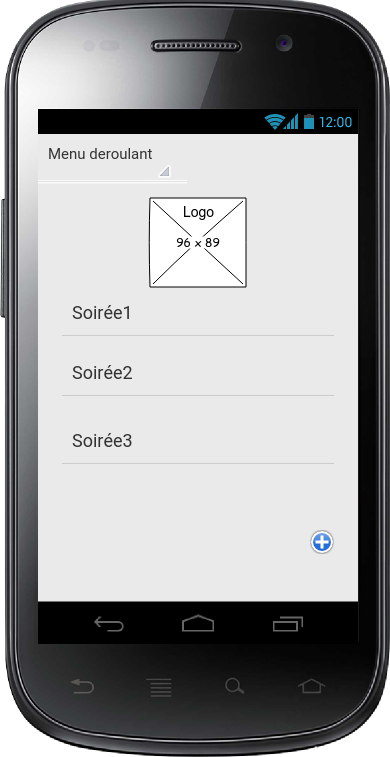
\includegraphics[width=0.7\textwidth]{accueil.png}
  \caption{Écran d'accueil}
  \label{Maquette:Accueil}
\end{maquetteFig}

\begin{maquetteFig}[!htb]
  \centering
  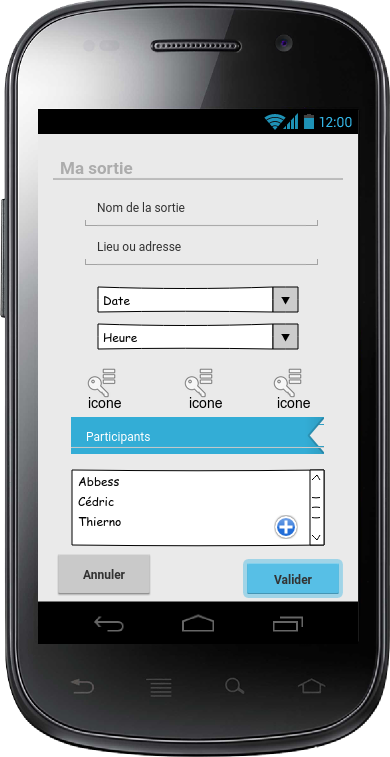
\includegraphics[width=0.7\textwidth]{creation_soires.png}
  \caption{Écran de création d'une sortie}
  \label{Maquette:CreerSoiree}
\end{maquetteFig}

\begin{maquetteFig}[!htb]
   \centering
     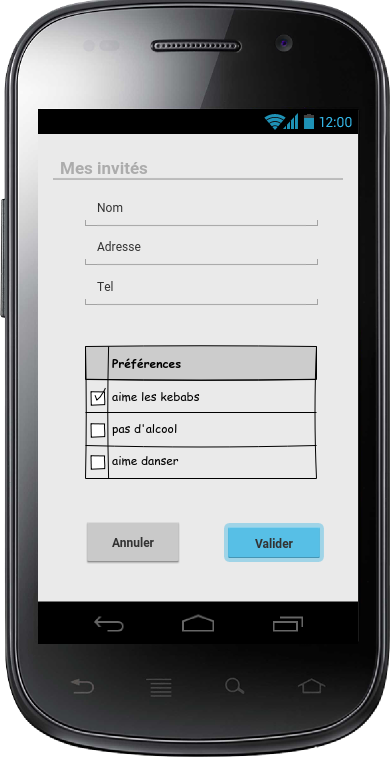
\includegraphics[width=0.7\textwidth]{ajout_participants.png}
     \caption{Écran d'ajout d'un participant}
     \label{Maquette:AjoutParticipant}
\end{maquetteFig}

\begin{maquetteFig}[!htb]
  \centering
     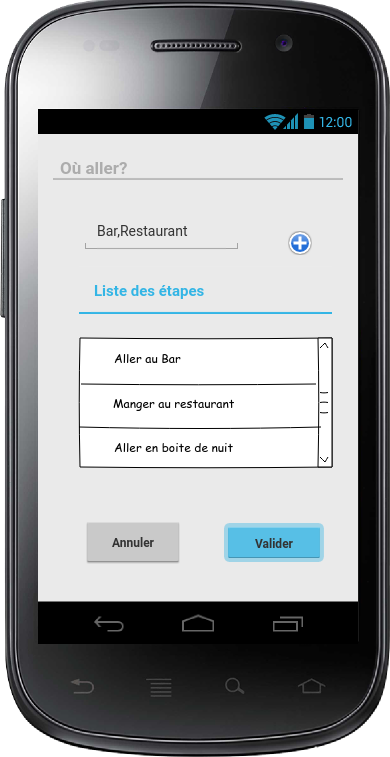
\includegraphics[width=0.7\textwidth]{ajout_lieux.png}
     \caption{Écran d'ajout de lieux}
     \label{Maquette:AjoutLieux}
\end{maquetteFig}

\begin{maquetteFig}[!htb]
   \centering
     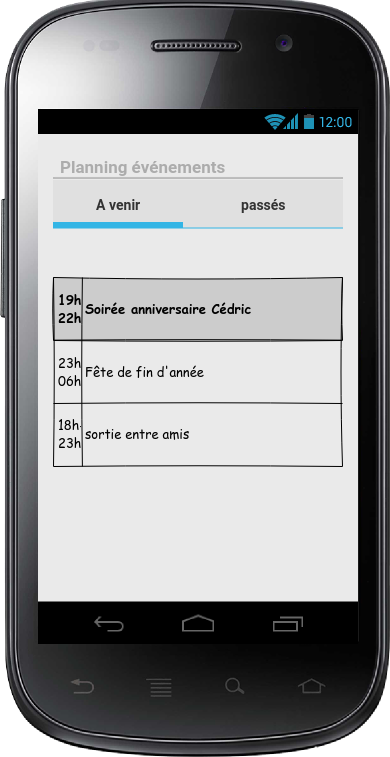
\includegraphics[width=0.7\textwidth]{planning.png}
     \caption{Écran d'affichage du planning d'une soirée}
     \label{Maquette:Planning}
\end{maquetteFig}

\begin{maquetteFig}[!htb]
  \centering
     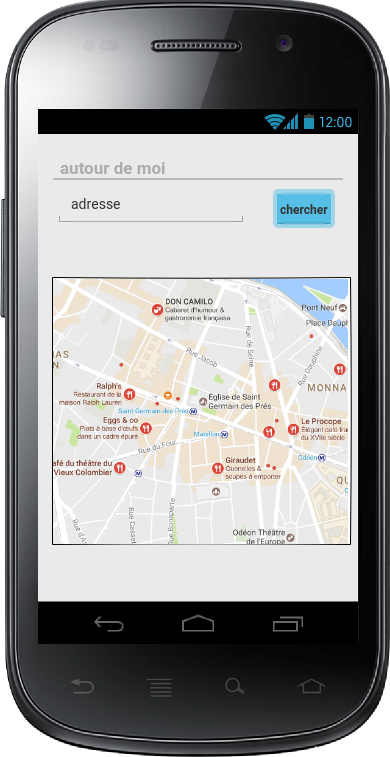
\includegraphics[width=0.7\textwidth]{autour_de_moi.png}
     \caption{Écran représentant les points d'intérêt "autour de moi"}
     \label{Maquette:AutourDeMoi}
\end{maquetteFig}

% On place ici tous les diagrammes UML
\begin{umlFig}[!htb]
   \centering
   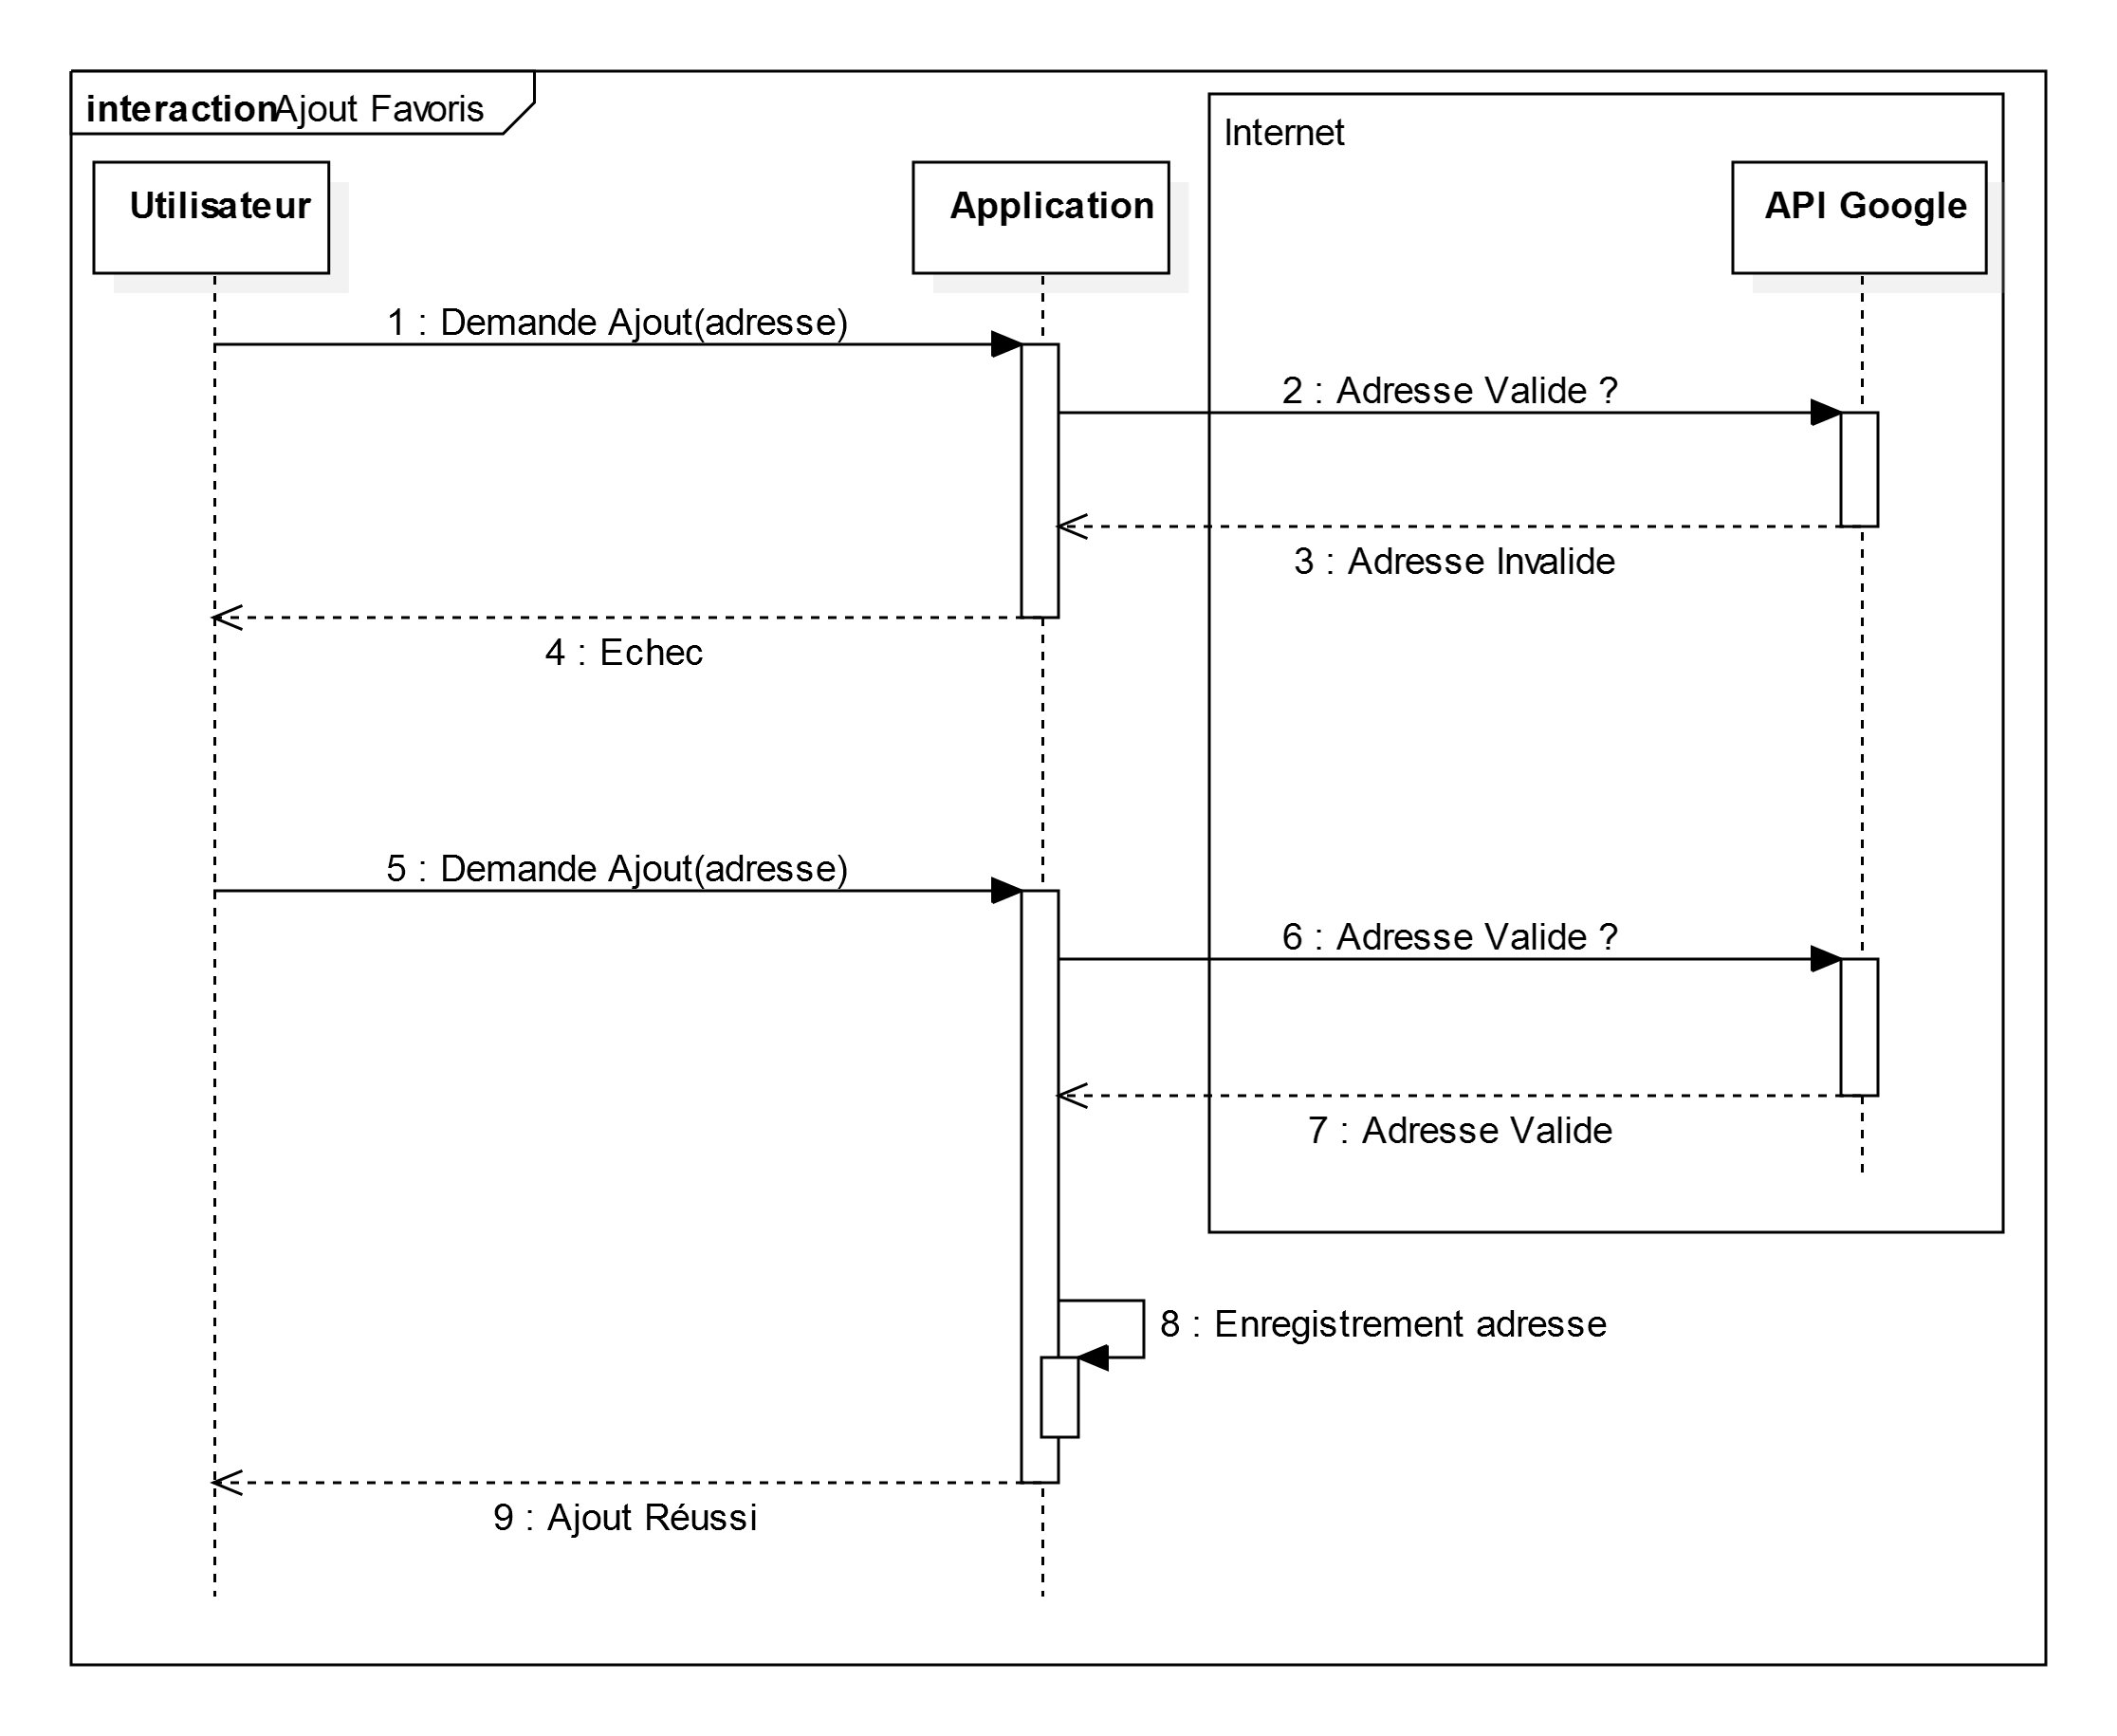
\includegraphics[width=\textwidth]{AjoutFavoris.png}
   \caption[Diagramme d'ajout d'un lieu en favoris]{Diagramme de séquence représentant le fonctionnement de l'application lors de l'ajout d'une adresse à notre liste de favoris. D'abord avec une adresse invalide (qui ne sera donc pas ajoutée), puis avec une adresse valide.}
   \label{UML:AjoutFavoris}
\end{umlFig}

\begin{umlFig}[!htb]
   \centering
   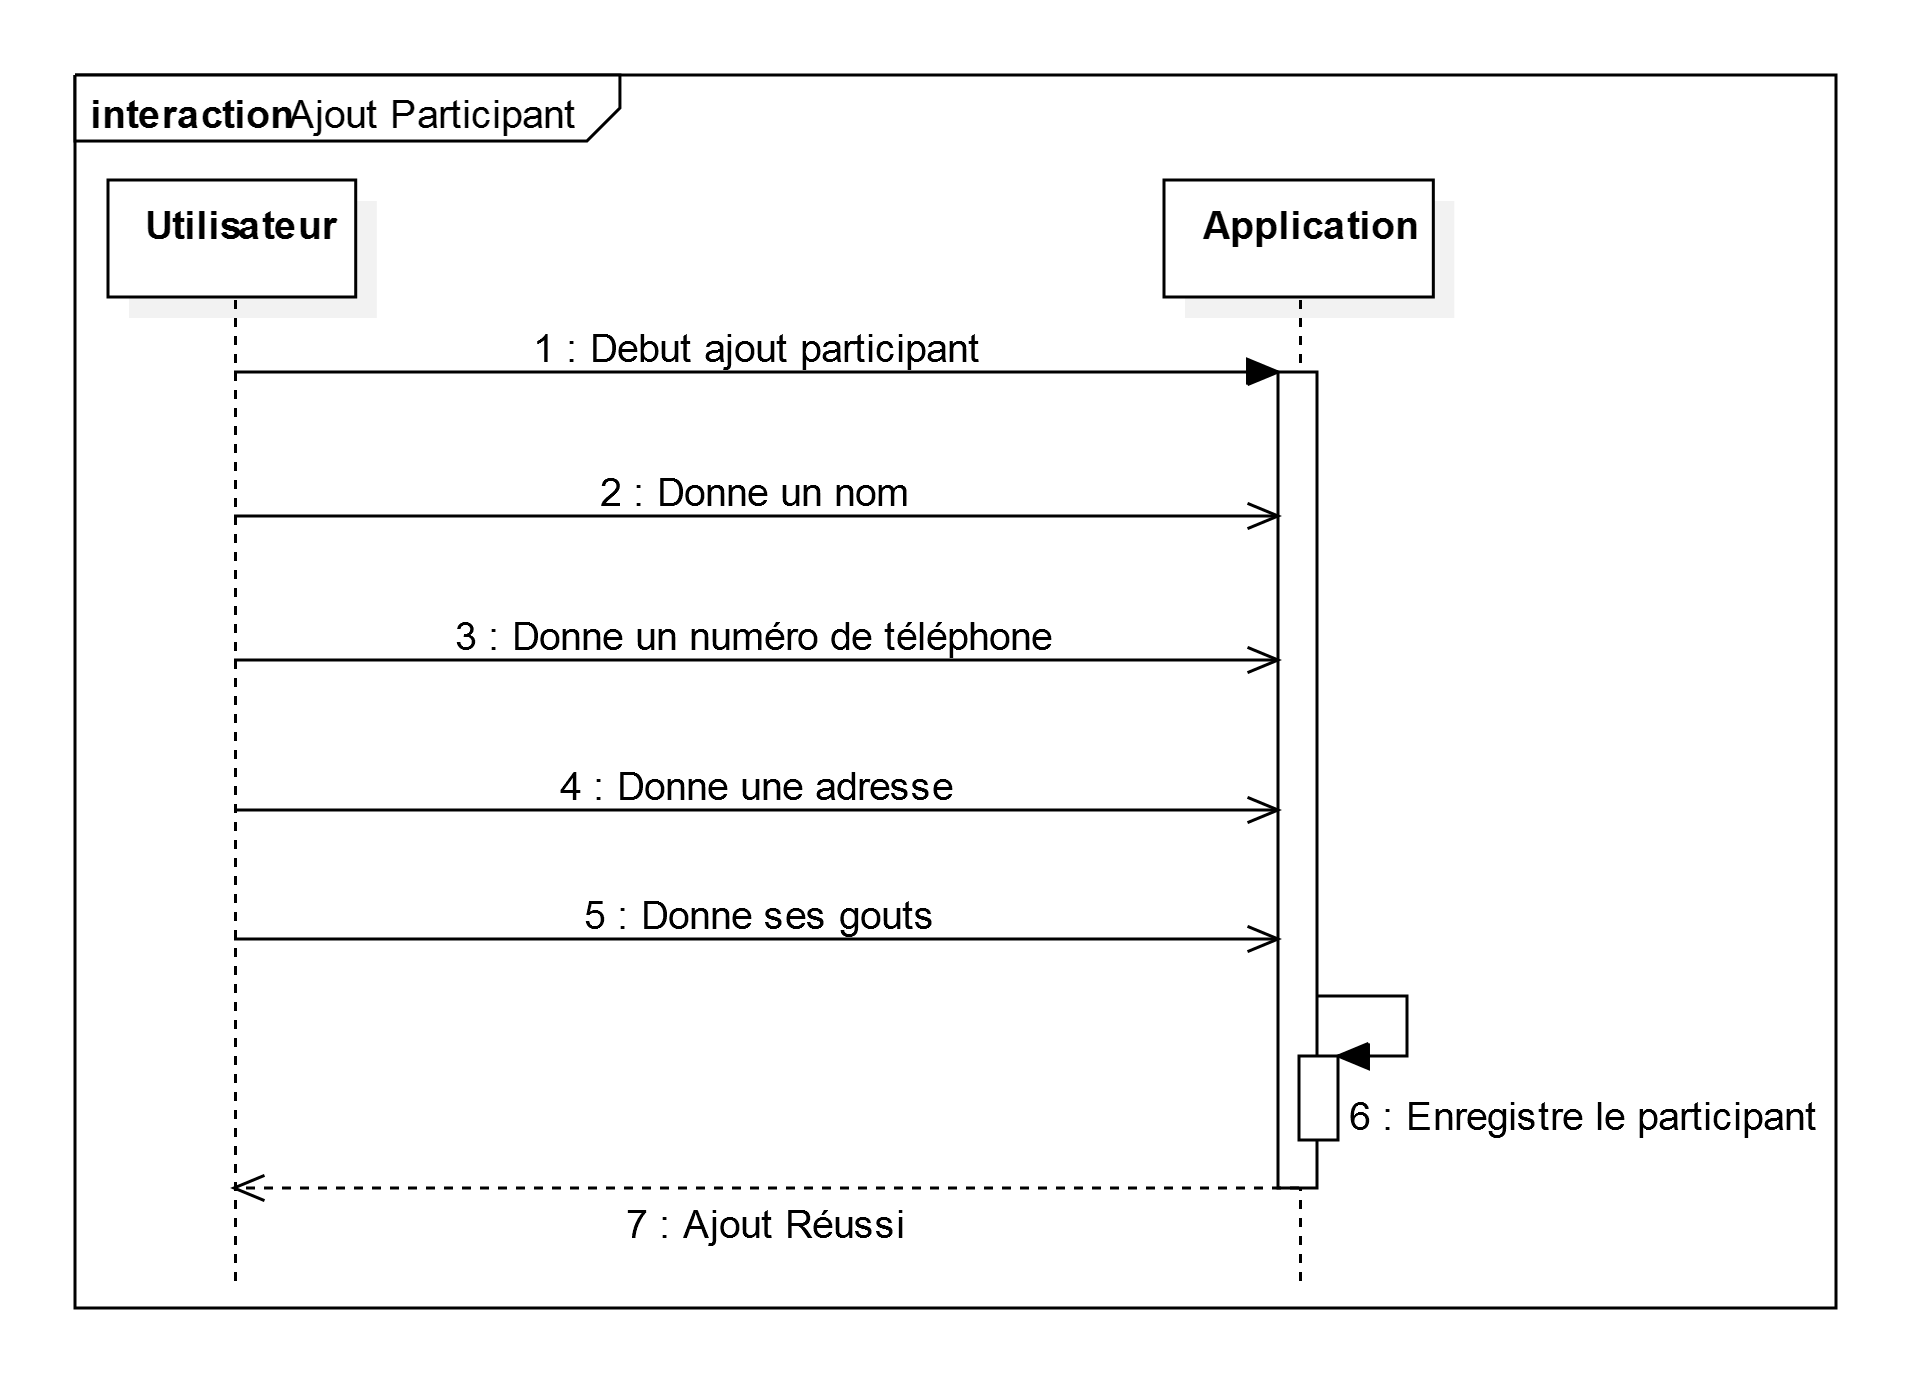
\includegraphics[width=\textwidth]{AjoutParticipant.png}
   \caption[Diagramme d'ajout d'un participant]{Diagramme de séquence montrant comment est ajouté un participant en renseignant la totalité des informations possibles sur cette personne.}
   \label{UML:AjoutParticipant}
\end{umlFig}

\begin{umlFig}[!htb]
   \centering
   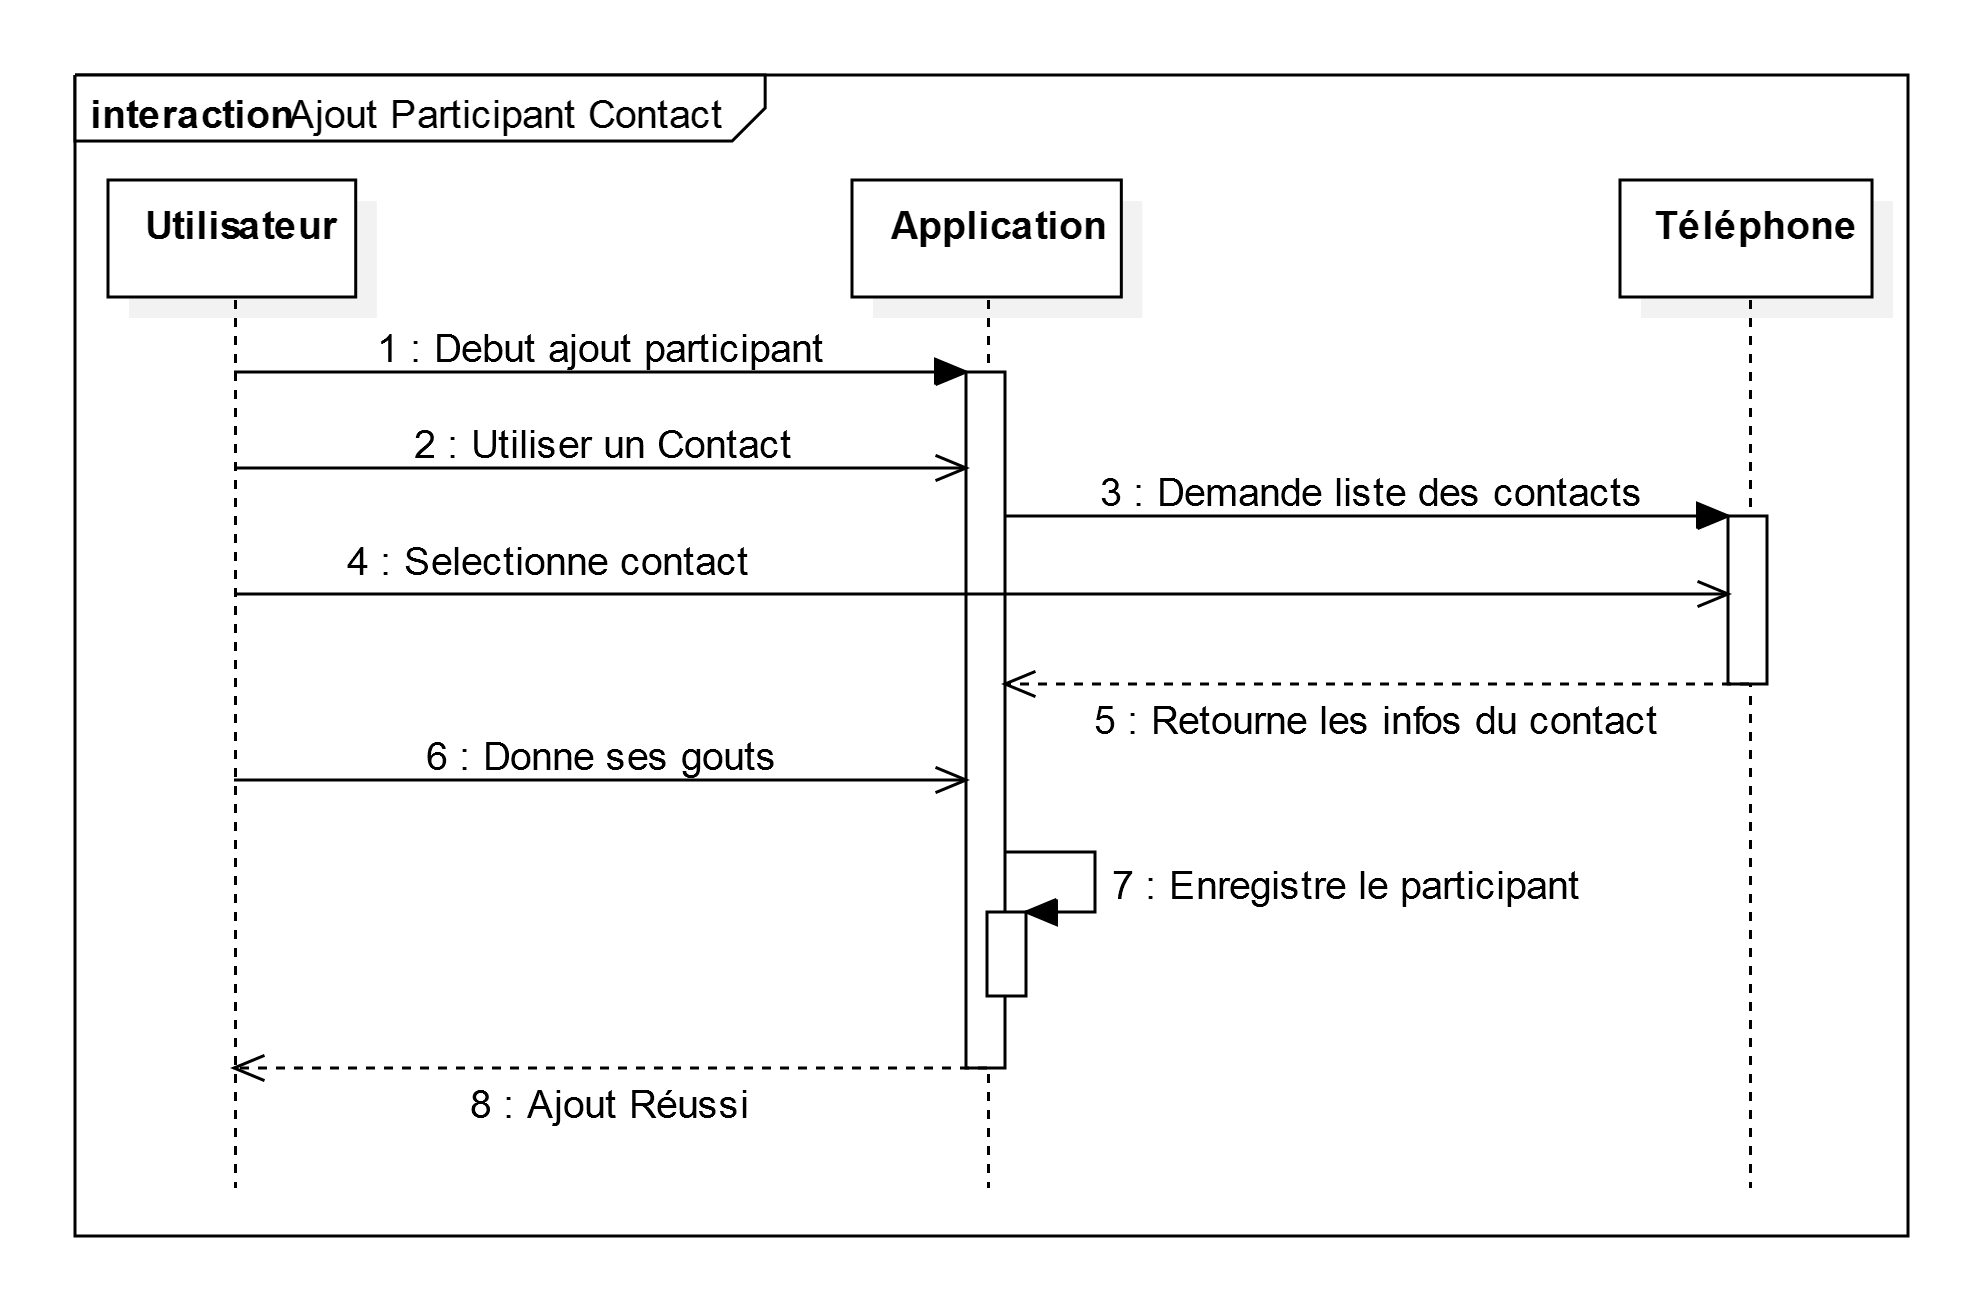
\includegraphics[width=\textwidth]{AjoutParticipantContact.png}
   \caption[Diagramme d'ajout d'un participant depuis ses contacts]{Diagramme de séquence montrant comment ajouter un participant à une soirée en utilisant la liste de contacts accessible sur le téléphone de l'utilisateur. Seuls les goûts du contact devront être ajoutés manuellement (si les autres informations trouvées conviennent).}
   \label{UML:AjoutParticipantContact}
\end{umlFig}

\begin{umlFig}[!htb]
   \centering
   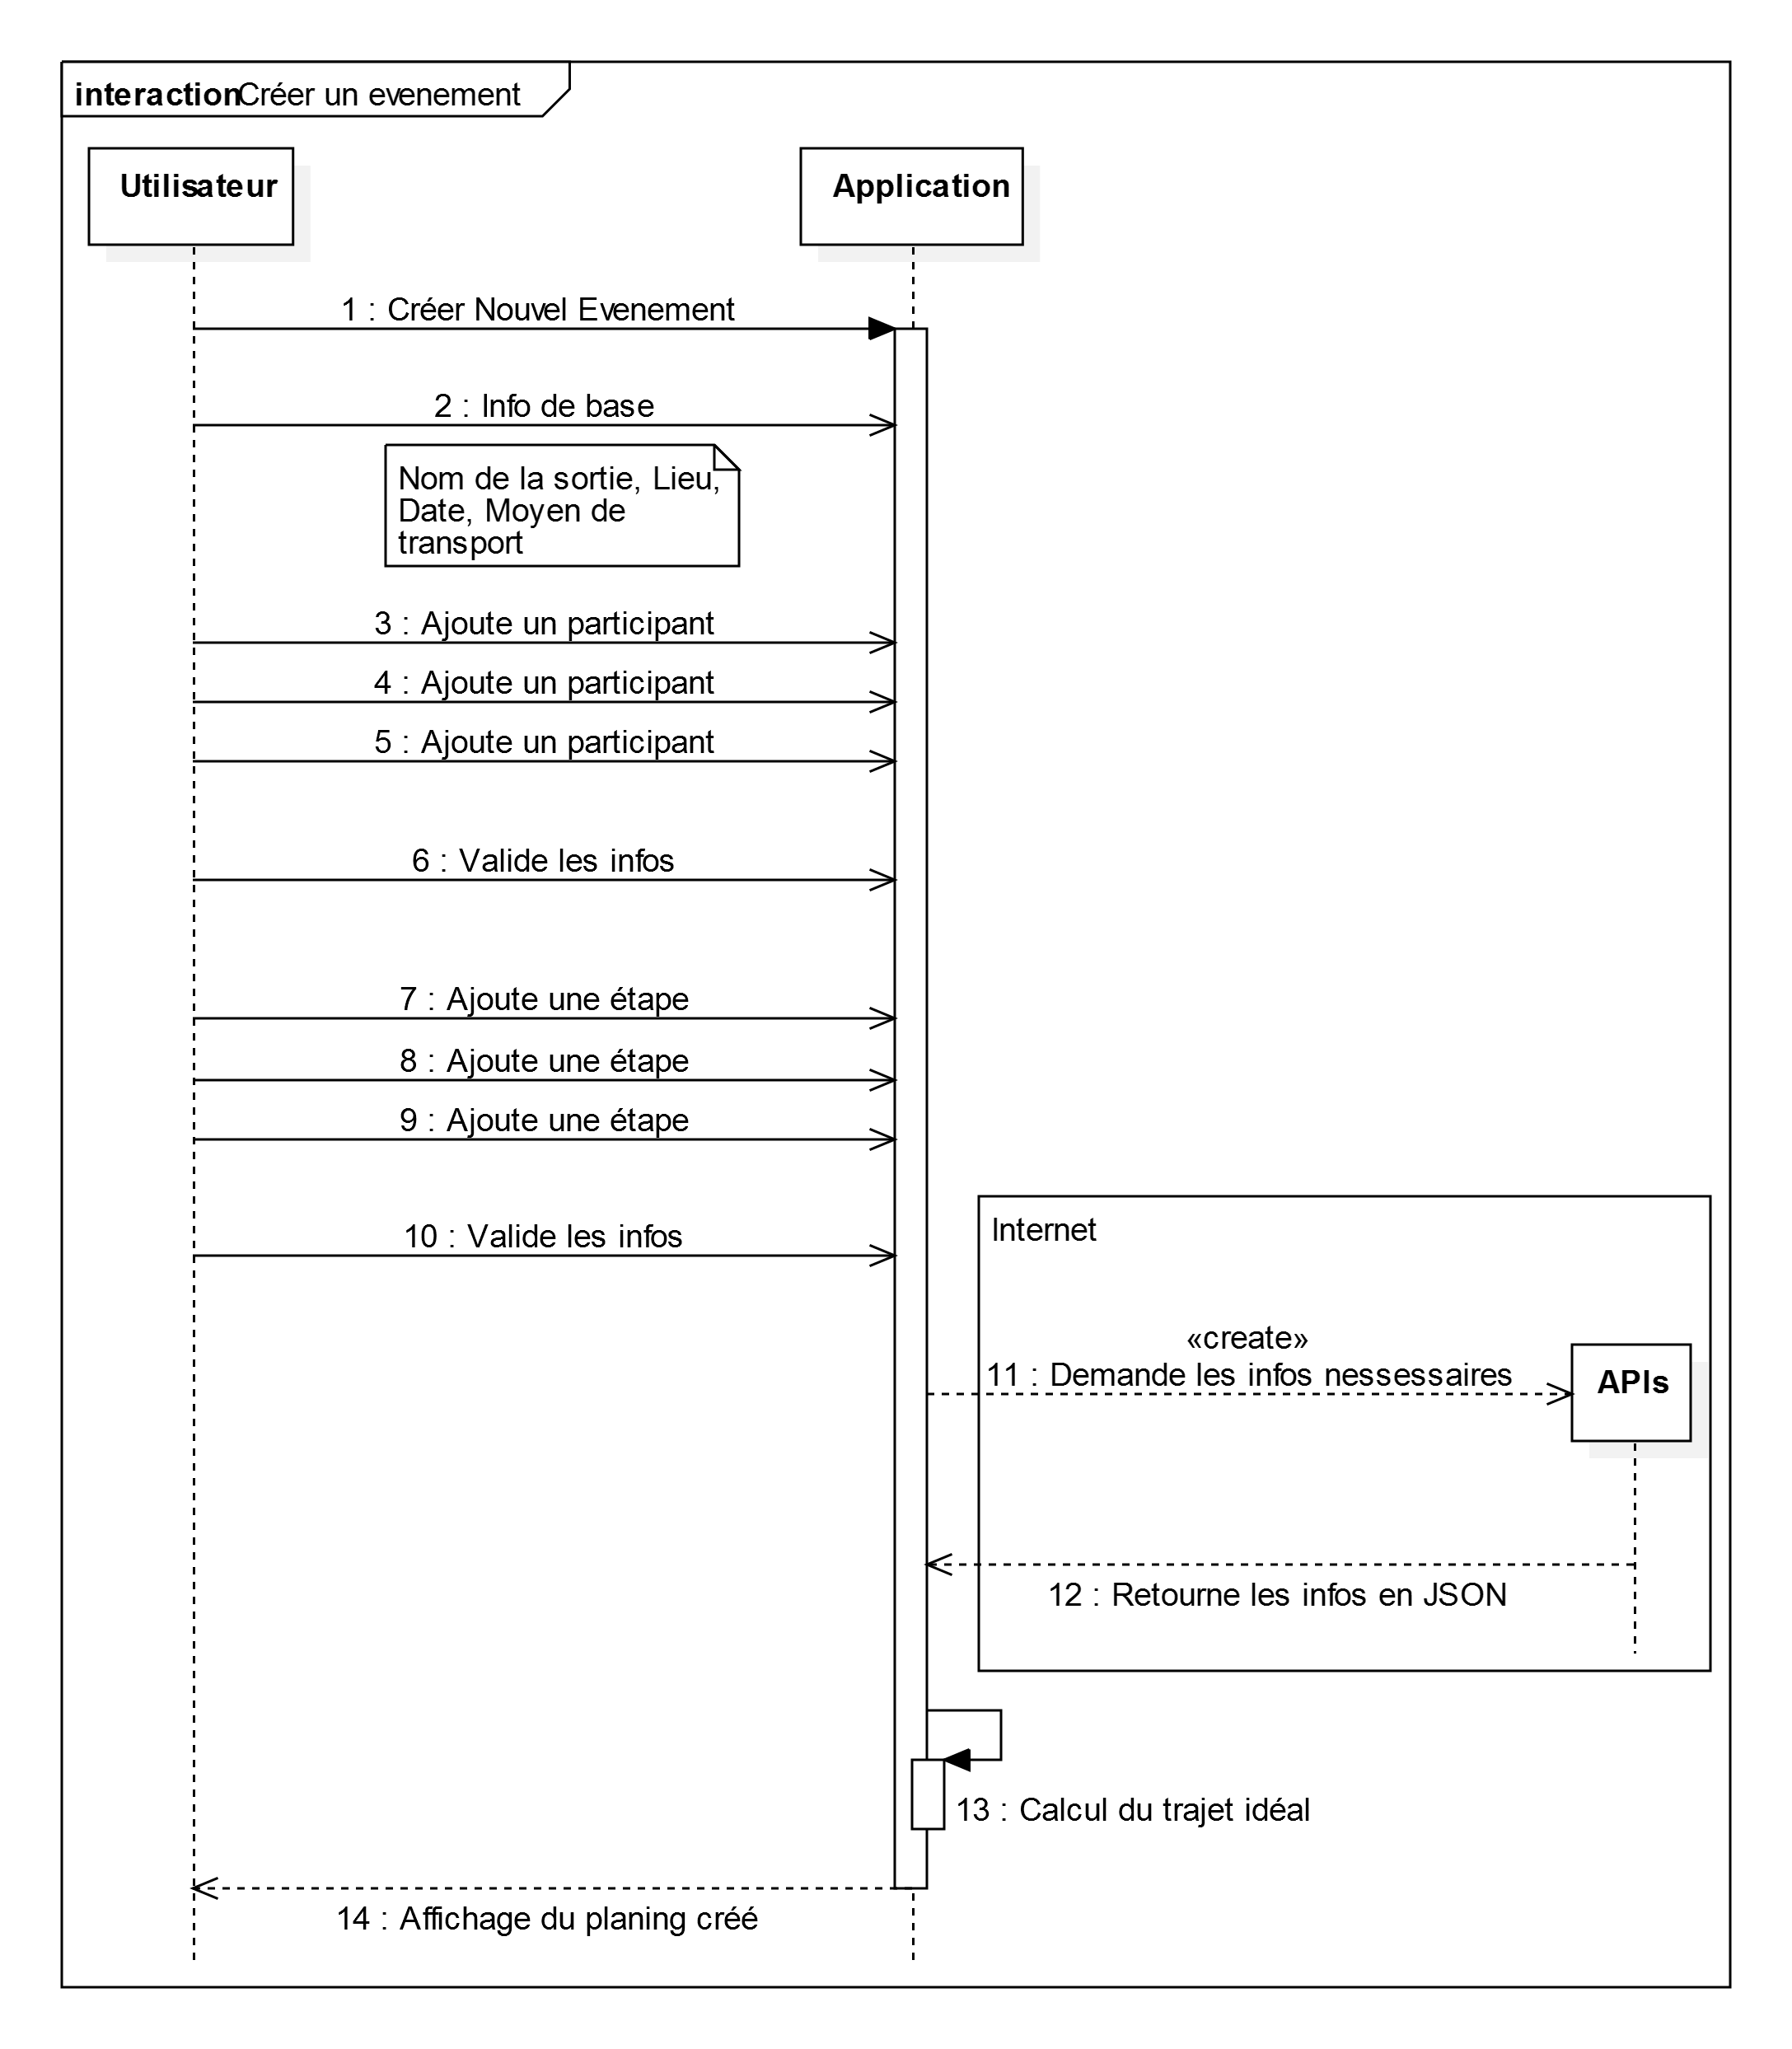
\includegraphics[width=\textwidth]{CreerEvenement.png}
   \caption[Diagramme de création complète d'un événement]{Diagramme de séquence représentant la création d'un événement du début à la fin en effectuant toutes les étapes dans l'ordre. Il peut évidement y avoir autant d'ajouts de participants et d'étapes que voulu.}
   \label{UML:CreerEvenement}
\end{umlFig}

\begin{umlFig}[!htb]
   \centering
   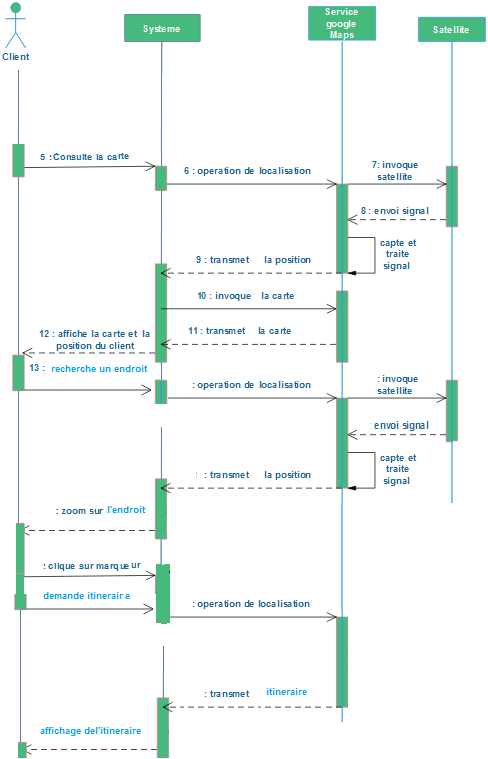
\includegraphics[height=0.9\textheight]{UtiliseMap.png}
   \caption[Diagramme d'utilisation de la carte]{Diagramme de séquence représentant l'utilisation de la carte pour faire plusieurs actions tel que regarder autour de soi, rechercher un point d'intérêt et trouver l'itinéraire vers ce point.}
   \label{UML:UtiliseMap}
\end{umlFig}

\begin{umlFig}[!htb]
   \centering
   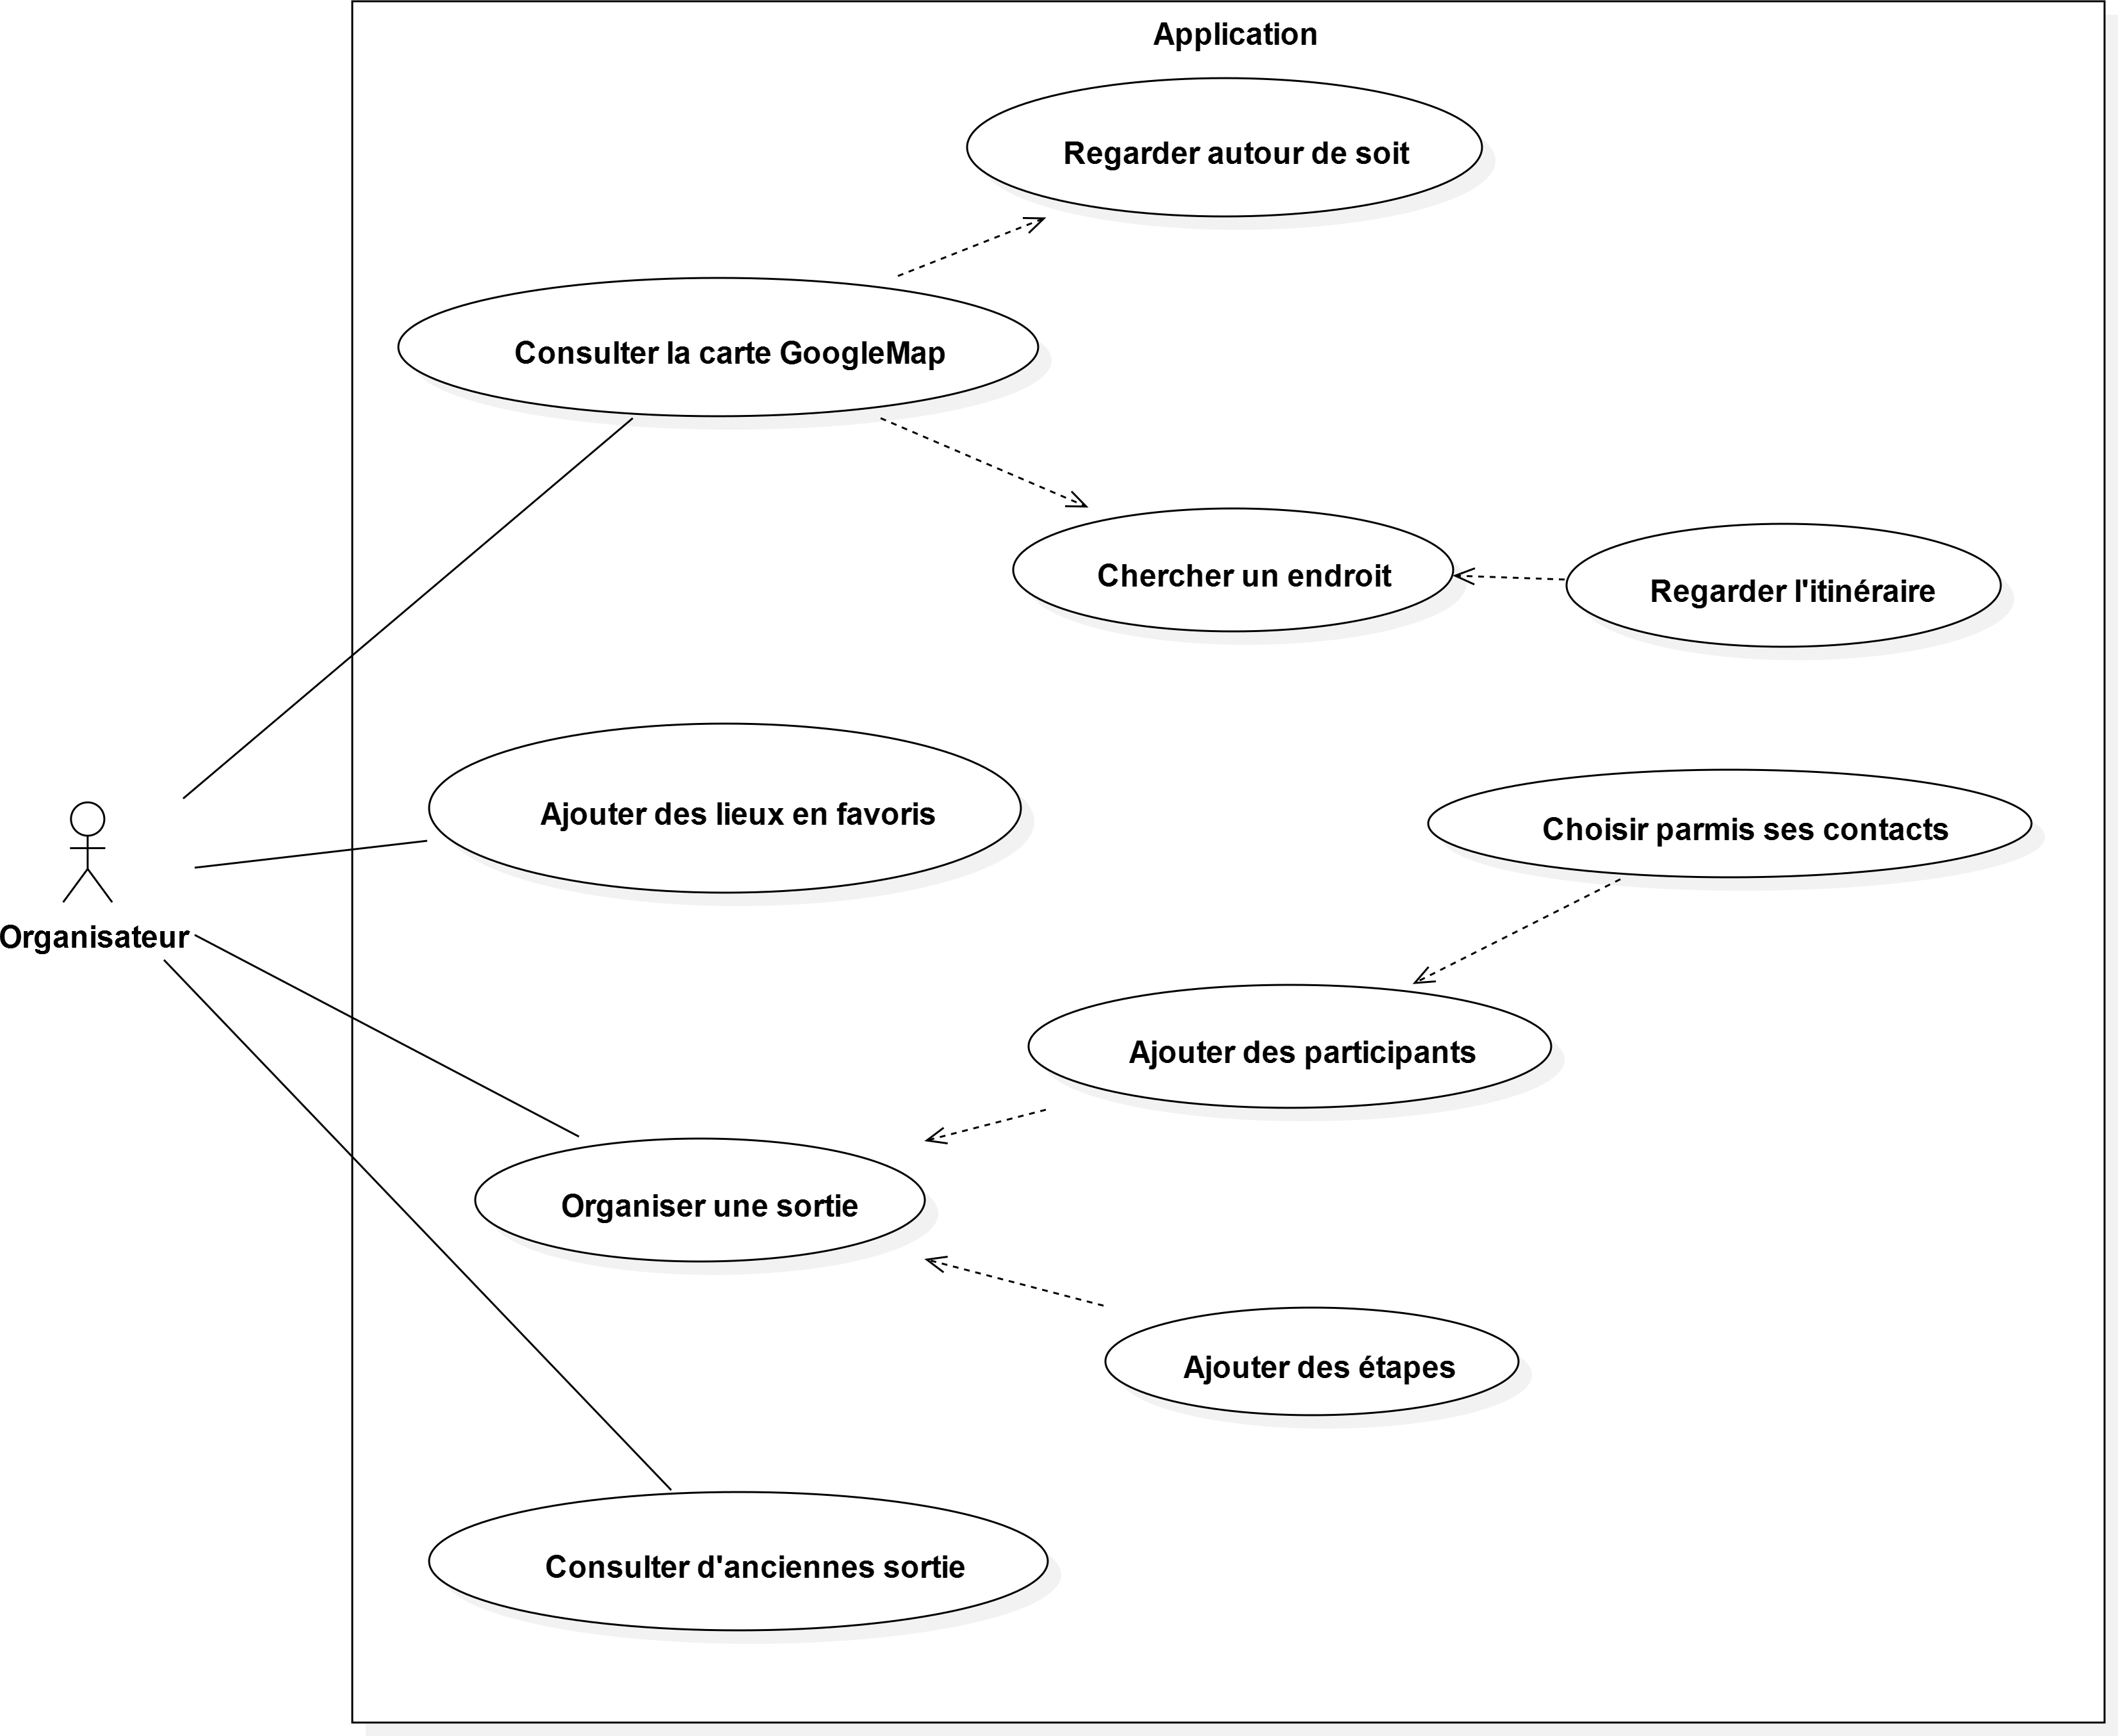
\includegraphics[width=\textwidth]{CasDutilisation.png}
   \caption[Diagramme des cas d'utilisation]{Diagramme des cas d'utilisation de l'application.}
   \label{UML:CasDutilisation}
\end{umlFig}

\begin{umlFig}[!htb]
   \centering
   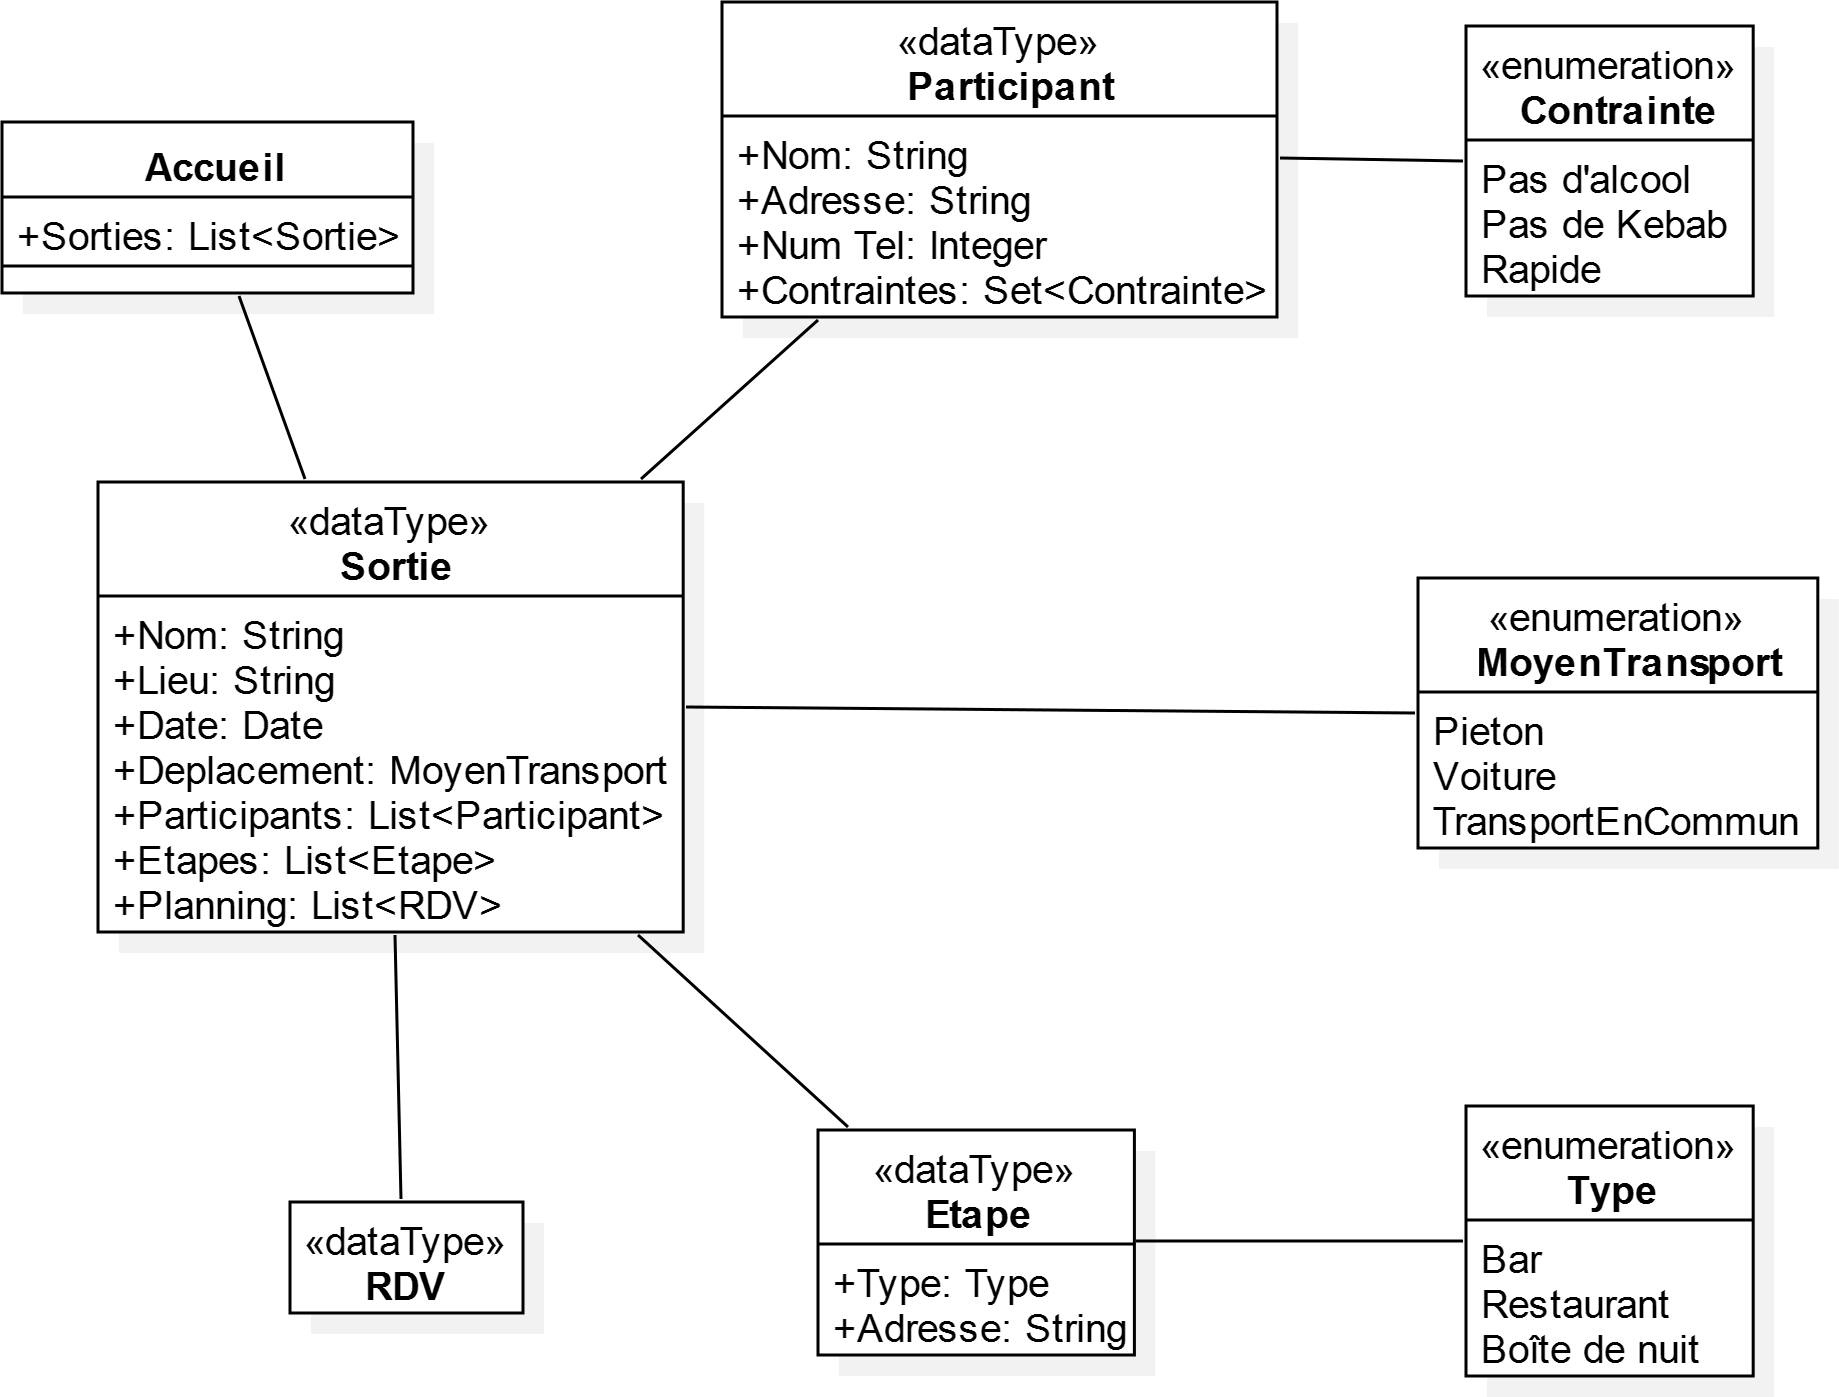
\includegraphics[width=\textwidth]{DiagrammeDeClasse.png}
   \caption[Diagramme de classe]{Diagramme simplifié des classes et de la structure de notre application.}
   \label{UML:Classe}
\end{umlFig}


\end{document}

\section{API utiles}
\begin{easylist}[itemize] \itemizePuce
& En rapport avec les transports en commun :
&& \url{https://www.navitia.io/} (pas encore inscrit mais semble bien marcher)

& Extraire des données d'OpenStreetMap :
&& \url{http://overpass-turbo.eu/} (une doc est dispo \href{http://wiki.openstreetmap.org/wiki/Overpass_API}{ici} et ça marche plutôt bien)

& API google pour affichage de cartes
&& \url{https://developers.google.com/maps/documentation/android-api/}

& Pour appeler un taxi (ou hubber)
&& \url{https://api.gouv.fr/api/le-taxi.html} (C'est pour les entreprises, il faut un numéro siret)
&& \url{https://developer.uber.com/} (Je n'ai trouvé nul part si c'était gratuit et libre d'utilisation)

& Pour trouver la localisation d'une adresse (ou l'adresse depuis une position) :
&& \url{https://api.gouv.fr/api/base-adresse-nationale.html}
&& \url{http://wiki.openstreetmap.org/wiki/FR:Nominatim}

& La météo locale (on a accès gratuitement à des prévisions sur 5 jours) :
&& \url{http://openweathermap.org/api}

& Pour utiliser son calendrier (apparemment réservé à l'API 23 ou plus) :
&& \url{https://developers.google.com/google-apps/calendar/}

& On peut parser les données d'Allociné pour avoir les horaires mais ça risque d'être relou.

\end{easylist}